\documentclass{acm_proc_article-sp}

% UTF8 encoding and scalable fonts
\usepackage[utf8]{inputenc}
\usepackage[T1]{fontenc}

\usepackage{microtype}
\usepackage{graphicx}
\usepackage{subfigure}
\usepackage{booktabs}
\usepackage{listings}
% url support with hyphen line break
\usepackage[hyphens]{url}
% clickable links for stuff with hidden markup
\usepackage[hidelinks]{hyperref}
% for \currenttime
\usepackage{datetime}
% better captions
\usepackage[font=small,labelfont=bf]{caption}

\begin{document}

\conferenceinfo{Human Computer Interaction Project – Media Informatics Display Network.}{\\Ulm University, Ulm, Germany.}
\CopyrightYear{2013}

% Change to your title
\title{MIND – Media Informatics Networking Displays \\ (Working Title)}
\subtitle{Evaluation of Interaction Considerations \\ {\normalsize \today \ – \currenttime} }

% Change to your personal details
\numberofauthors{4}
\author{
\alignauthor
Andreas Köll\\
       \affaddr{Institute of Media Informatics}\\
       \affaddr{Ulm University}\\
       \affaddr{Ulm, Germany}\\
       \email{andreas.koell@uni-ulm.de}
\alignauthor
Laura Irlinger\\
       \affaddr{Institute of Media Informatics}\\
       \affaddr{Ulm University}\\
       \affaddr{Ulm, Germany}\\
       \email{laura.irlinger@uni-ulm.de}
\and
\alignauthor
Patryk Boczon\\
       \affaddr{Institute of Media Informatics}\\
       \affaddr{Ulm University}\\
       \affaddr{Ulm, Germany}\\
       \email{patryk.boczon@uni-ulm.de}
\alignauthor
Tamino P.S.M. Hartmann\\
       \affaddr{Institute of Media Informatics}\\
       \affaddr{Ulm University}\\
       \affaddr{Ulm, Germany}\\
       \email{tamino.hartmann@uni-ulm.de}
}

\maketitle

% Intro
\section{Introduction}

We propose a system for liquid transfer of applications between physical and virtual hardware devices.
To facilitate this functionality, we will take a closer look at the applications, devices, and hardware components available to us.
% System types
In the following we will take a look at the possible system, application, and human interaction possibilities.
We will evaluate and categorize the different system to person combinations for their usability as a human-computer-interaction project.

Regarding a multi-user system, there are different entity-relationships to be considered, each with its own concomitant features.
In the following, the entities described in the relationships are the intended endpoints or terminal devices of the connections.

Among the most common relationships is the link between the user and the system, short \textbf{one-to-system}.
This connection implies e.g. a user storing data, such as appointments in her/his calendar, to be accessible afterwards.

A further relationship is represented by the link between two users, hence \textbf{one-to-one }relationship.
This configuration is commonly used for transferring data between two users or alternatively two devices.
Such a communication can provide a high level of privacy, provided each device represents one user, e.g. when using smartphones.

The \textbf{one-to-many} configuration represents a scenario in which, starting from one terminal device, a broadcast is sent to a pre-defined compilation of devices.
This phenomenon is omnipresent in respect of social networking, thus rendering this configuration extremely common - with all its concomitant privacy issues.

The \textbf{system-to-one} link describes a relationship where the interaction is invoked by the system and provokes output on one terminal device.
This can be implemented pre-setting a date and time, registering a certain change in the environment using sensors or triggering a notification message to be sent after finishing a computing task.
In an extreme case, this configuration doesn’t require any interaction with the user, however the output may show a deficit in the matter of privacy, for instance when the user receives private information while not interacting with the device.
This effect may even be enhanced when the information is sent to a more or less public display in a network of displays.

The \textbf{system-to-many} relationship can be rated similar to the system-to-one configuration, with an even greater loss in privacy - since potentially confidential information might be received by multiple devices without the proper recipient on site.
Possible applications involve reminders for group activities and clues about changes in the environment, such as emergency notifications.

A \textbf{many-to-many} relationship ordinarily applies in network gaming or (video) conferencing. Although privacy issues may arise from such a configuration, it enables simultaneous interaction of multiple users.
% related work
\section{Related Work}
% Mit bold, jeder einen Absatz
The following section contains an overview of related work, categorized in the possible system types.
%The following section contains an overview of related work. First research about system types is collected. Afterwards an overview about possible input interactions is given, followed by related work about output. Lastly some papers about networking are granted.

\subsection{General}
\paragraph{Modeling multimodal human-computer interaction}
Obrenovic and Starcevic \cite{obrenovic_modeling_2004} observed modeling input and output modalities using UML2.
According to them input modalities can be categorized as streaming-based and event-based.
Event-based input modalities are for example input via a keyboard or mouse, streaming-based input is for example input from sensors (microphone etc.).
They also differentiate between two general types of output.
Static and dynamic output.
Static output is for example a picture, dynamic output a video.
Some forms of dynamic output therefore consist of animated static output.
Another topic they discuss is the response time of systems.
There is the socalled perceptual processing time (< 0.1sec) which appears to a person instantaneous and multiple such events as continuous.
There is the immediate response time (~1sec) which is the minimum time a person requires to react to a new situation and there is the unit task time (~10sec) which is the scale for the simplest tasks the person wants to perform.

\subsection{One-To-One}

\paragraph{Clearing the Virtual Window - Connecting Two Locations
with Interactive Public Displays }
Häkkilä et al. \cite{hakkila_clearing_2013} investigate notifying the other end for a live video feed connection between two locations via public displays.
Each window represents a frozen widow to the other room.
By using gestures the ice could be melted from both ends allowing visual communication.
In their study using a two-sided ice melting design was most comfortable for their participants as communication attempts could be seen but also the privacy was respected.

\subsection{One-To-Many}

\subsection{One-To-System}

\paragraph{Exploring the utility of remote messaging and situated office door displays}
Cheverst et al. proposed \textbf{remote messaging and situated office door displays} \cite{cheverst2003exploring}.
Dating back to a time when SMS was extremely prominent, this work investigates the utility of sending messages not to a particular cellphone owned by a person but to one displays situated at particular locations.
One purpose of such an implementation was to explore whether a digital alternative is an enhancement to traditional post-it notes.
The owner of a display can leave a message on the display itself, via a web interface, an email client or by SMS messages.
Messages left by visitors can be entered at the display.
Those messages, however, are not visible for visitors due to privacy and spatial reasons.
The owner can read messages on the display itself, through a web interface or email, thus rendering such an implementation as one-to-system or system-to-one system type.
An extension of visitors’ interaction with office displays is introduced by Cheverst et al. in \cite{cheverst2005exploring}, describing the usage of Bluetooth as an in- as well as output channel for visitors.
Additionally to leaving a message, visitors can download certain data from the display owner.
With the limited range of Bluetooth, the visitor has to approach the display to a few meters, which might be argued to be an inconvenience since data can be obtain using the internet, as well.
However, according to \cite{cheverst2005exploring}, owners of data are more willing to share (more private) data with visitors who have made the journey to their office.

\paragraph{Lean and zoom: proximity-aware user interface and content magnification}
Harrison and Dey \cite{harrison_lean_2008} use the user's proximity to a screen and their leaning pose to determine the size of the information to be displayed.
Leaning forward resulted in a proportional magnification of the screen's display.
In their study participants found that items on screen could be read easier an more comfortably using this technique.

\paragraph{Mobile applications for open display networks: common design considerations}
José et al. \cite{jose_mobile_2013} look at ways a user can interact with public displays using his mobile device.
This includes creating the association between mobile device and display, using the device as controller and transmitting data.


\subsection{System-To-One}

\paragraph{Ambient Displays: Turning Architectural Space into an Interface between People and Digital Information}
Wisneski et al. \cite{wisneski_ambient_1998} create an ambient room and take a look at what possible mapping techniques there are to represent different types of information to the user. They use light, sound and movement to inform the user in a subtle way.

\subsection{Many-To-Many}

\paragraph{The Interacting Places Framework: Conceptualizing Public Display Applications That Promote Community Interaction and Place Awareness}
Memarovic et al. \cite{memarovic_places} describe potential \textbf{public display} applications to foster community interactions.
This work considers applications for a public display scenario and proposed a framework for implementation purposes.
Potential applications comprise e.g. transmitting text or (Flickr) images to a public display to be shown.
In addition, social media content can be displayed such as twitter feeds or facebook sites.
Aside from that, content can be service provided and does not have to originate from users.
This includes bus schedules, advertisement or other location based information such as the weather forecasts or upcoming events.
Such a mode can be described as a system-to-one or system-to-many system type with the output being initiated by the system itself.
Among the possibilities for producing the to-be-displayed content are the publishment of information via smartphone, email, social media or a simply by dropping the content in a network folder.

\paragraph{Screen Codes: Visual Hyperlinks for Displays}
In order to distinguish multiple interactions on public displays, Collomosse and Kindberg \cite{Collomosse_ScreenCodes} proposed C-Blink as visual-based interaction channel. The screen of the user’s smartphone emits a sequence of colors which represents coded information. The sequence is seized by a camera mounted on the public display, thus encoding the information.

\paragraph{Yarely: a software player for open pervasive display networks}
Yarely is a software player designed by Clinch et al. \cite{Clinch_Yarely} which is based on pervasive display networks. Whereas conventional media players are controlled by one authority, Yarely is supposed to perceive content as well as a play out schedule from several sources simultaneously. The actual output of content will be evaluated by the player itself.
One design goal of Yearly was extensibility. The integration of new components, e.g. adding environmental sensing for input purposes or rendering of the displayed content, is intended to cause minimal changes to the core player.


\subsection{System-To-Many}

\paragraph{Crossmodal Attention in Public-Private Displays}
Olivier et al. \cite{Olivier_Crossmodal} propose CrossBoard, where the user’s smartphone is synchronized with the public display.
In order to distinguish information that is relevant for the user, the display highlights pieces of information periodically while the user’s smartphone vibrates as long as the relevant information is highlighted.

\paragraph{Interactive Public Ambient Displays: Transitioning from Implicit to Explicit, Public to Personal, Interaction with Multiple Users}
Vogel et al.\cite{Vogel_InteractivePublicAmbient} exploit body tracking to determine which information should be displayed on which section of big public screens. Position (proximity to the screen) as well as posture of the user indicate the size and position of the relevant section of the display while RFID tags or face recognition is applied for identification and selection of information.

\paragraph{Visual Highlighting on Public Displays}
Ostkamp et al. \cite{Ostkamp_VisualHighlighting} introduce AR-Multipleye as an AR-based approach for visual highlighting using smartphones. A QR tag is situated on the public screen and provides information about different visual highlightings. A hint for the relevant information may e.g. be a transparent overlay on the piece of information when seen through the smartphone’s camera.

% many to system <-> system to many?
\paragraph{Proxemic Interaction: Designing for a Proximity and Orientation-aware Environment}
Ballendat et al. \cite{ballendat_proxemic_2010} take the concept of proxemics further and develop a proxemic media player which reacts to the angle, movement and view of one or multiple persons in front of a ambient display.
So looking away from the monitor pauses the movie, moving towards the display shows more information the closer the person is to the display.
E.g. from far away an overview of running movies is shown.
From closer up also information like its title is shown.
Sitting on the couch toggles the movie fullscreen.
A second user approaching the display is shown the title when away and a detailed information in a split screen view when close to the display.
The second view continues playing the movie.

\paragraph{Ambient displays and mobile devices for the creation of social architectural spaces}
Streits et al. \cite{streitz_ambient_2003} show a public display called Hello.Wall to show information about people in it's proximity.
They differentiate between Interaction, Notification and Ambient Space which allow different interaction with the display.
This information is also used to be transmitted to a remote identical display and thus enhancing people in a remote place discretely about knowledge of the other location.
This knowledge includes the general mood obtained from mobile devices (View.Port) associated with each person and can be used to see if there is the will for a video conference.
The mobile device also functions as private output when within interaction zone of the display.
Private information is otherwise coded in a abstract symbol on the display itself notifying the user associated with it about its existence.




\subsection{Input}
Nacenta et al. \cite{a18-nacenta} introduced a multi-user system called LunchTable.
Often people in groups check information on their mobile devices during conversations (for example during lunch). But for sharing information in groups mobile devices are less suitable: displays are simply too small.
Large displays are easily shared by multiple users. So interaction in groups shall be simplified by a multi-user multi-display system: the LunchTable.
The prototype uses a vertical display on the wall and a multi-touch display embedded within a regular lunch table.
The information on the display can be controlled via the multi-touch display.
The users can manipulate the wall display space by interacting with the horizontal surface window manager (LunchTable).
Windows, also several simultaneously, can be manipulated by dragging their thumbnail. Moving application tiles into the regions of the window manager results in opening them on the display.
For a simple interaction with the display there are virtual input devices on the lunch table (trackpad and keyboard).
They can be opened with a trackpad icon and are connected to the thumbnail of the application.

Boring et al. \cite{p161-boring} used the mobile phone as an input device for large public displays.
They introduced three different interaction techniques: Scroll, Tilt and Move. With that the user can continuously control a pointer located on a remote display.
To move the pointer on the large display a user can press the joystick on the phone in the desired direction (Scrolling).
A user can accelerate the pointer by tilting the phone in the favored direction (Tilting).
Lastly the mobile phone can be used like an interactive laser-pointer (Moving).
Bidirectional interaction (input and output together) is possible using these techniques.
A study showed Move and Tilt to be faster but more error prone techniques for selection tasks compared to Scroll.

According to Baldauf et al. \cite{a4-baldauf} a camera-based control of large markerless displays through smartphones is a novel interaction technique.
To enable this for a large network of screens they implemented a prototype framework.
Hence the smartphone has to be able to register itself at one display (for example with a wireless connection).
So input commands can be communicated.
Afterwards the display and the smartphone periodically exchange image information.
Such the relation between the display and the mobile phone can be defined and so touch interactions on the mobile phone can be executed.


\subsection{Privacy}

This subsection lists related work concerning to privacy aspects of displays.
This will include public displays and display networks.

One way of allowing privacy on a single display is by restricting the content that can be viewed into angled field of views.
This is useful in the instance where a shared horizontal display is being utilized, such as a display table.
Whenever multiple users are present, viewing private data is not possible without making it visible to others.
One way of allowing the separation of private and public data can be achieved by a display mask that allows a single display to serve multiple views, as seen in \cite{smith2008public}.
In the paper, the authors present a working mask that allows public and private data to be shown together on a per user basis.
Public data is simply shown on all separate views (copying it to their framebuffers), while private data remains viewable to only the single originating instance.

Another interesting way of handling private and public aspects is found in \cite{baldauf2012private}.
Here, the public display serves as a common selection interface, while mobile devices are used to view the selected videos in a private way.
Baldauf et al. note that smartphones are now a common companion and thus well suited to be used as a private controller and display for interaction with public systems.
The paper also states that using the smartphone display as the private output was preferred over a competitive mode, where control of the public display was contested by the various users for showing a video.

\cite{shoemaker2001single} points out that one of the problems of using personal devices as the personal space is that the user has to divide her attention between multiple devices.
It is stated that this results in unnecessary cognitive overload for the user.
The paper shows a system that allows private information to be shown on a public display by utilizing shutter glasses and separating the content on the public display by timing the frames to the respective user's glasses.
The authors found the method to work well and to have a good acceptance.
Some of the questions raised include the question whether it is important to support private work in a collaborative setting; and how to signal to the user which data object is private and which is publicly viewable.

Another approach to hiding private, sensitive data is shown in \cite{1392750}.
Here, sensitive information is blurred out on the public display.
To view it, the user utilizes for example their smartphone like a flashlight, showing the clear text on their private display.

\cite{terrenghi2009taxonomy} raises the possibility of an ecosystem of displays that could be useable in social contexts.
The paper notably lists some insights that were gained.
Foremost of these for our own work is that the physical size of displays influences how they can be tied into a display ecosystem.
The authors also note that the effect of parallelism of tasks and their duration should be considered.
The conclusion is that future development should always remain aware of the social context, to best ensure a mature work environment.

\subsection{Networking}

Ian F. Akyildiz et al. \cite{akyildiz2005survey} give a good introduction to \textbf{mesh networks}.
They highlight where such networks might be useful, the advantages of using meshes, and also note the problems that still need to be solved.
The two main hurdles to overcome are robust scalability and security.
Scalability is required for a large number of mesh devices; security is important because the mesh devices shouldn't be trusted as a user has no control over them – they are not a trusted third party.
However since the above paper has been published, new research and new implementations have made significant steps towards solving some of these problems.
One example of such a possible solution is the Hyperboria \cite{hyperboria} project.

Some good questions pertaining to networking for \textbf{multiple display networks} are posed by Ferreira et al. \cite{ferreira2012scalability}.
The question, whether the same web standards will apply, and whether display networks will affect network performance should be considered in future work.

The survey by L. Atzori et al. \cite{atzori2010internet} concerns itself with the so-called \textbf{internet of things}.
In it the authors note that any advancement for an internet of things (henceforth IoT) must come from a wide range of topics, such as telecommunications or social sciences; this is also the case for our project.
Another aspect that might be of note is that the IoT includes an environment where smart objects interact with each other, much like computers do via the internet.
The survey highlights that a possible next step for the development of networks is away from the virtual space to a more physical one.
However, a range of technological and social issues will need to be addressed before that becomes a feasible future.
The main issue as stated are scalability and efficiency.

% GIA
The most basic interaction aspect we have to consider is whether interaction is active – meaning initiated by the user – or passive – meaning that the system reacts to stimuli apart from direct user input.
This has profound consequences for how the system would work and what it can be used for.
For example some tasks only work well with direct interaction, no matter the capabilities of the system, such as text input.

Apart from active or passive interaction we have to consider whether the system will work via a WIMP interface or if it will use a more metaphorical physical interaction scheme.
WIMP is the standard for computing and widely in use; no mental work is required when switching to the system if that is used.
A physical representation however is more intuitive.
Nevertheless, no standards exist (meaning most systems that are based on that work differently) and the discrepancy between the representation and the real world will always be a limiting factor.

Another aspect that needs to be considered is how and if we differentiate between multiple users per device.
This aspect has to be considered for targeting output and for identifying input and is called proximal regions.
For example if only one person is in a room we can use the complete room for input and output without differentiation.
If multiple users are within a room we will possibly be required to differentiate to the best of our capabilities based on the input and output hardware capabilities.
These capabilities are hardware dependent and therefore listed in the upcoming sections.
Independent of that, this decision is mainly influenced by the task the system will fulfill (meaning is differentiation required or can it be ignored?).

\subsection{Input – Interaction Spaces}

From an interaction standpoint, we can classify the different input possibilities for their distance to the device that will receive the input.

The first category is input \textbf{directly on the device} (as comparable to personal or intimate spaces in proxemics \cite{}), for example with the nowadays popular touch screen technology.
With a capable device, this input method allows fast and direct feedback that is immediately apparent to the user.
For software, designed for this input type, natural mappings can be used to create a very natural interaction.
This can however quickly break down for more complex tasks, as modern tablets and smartphones have shown – they are only easily useable for consumption tasks and not for tasks that require a more complex interaction flow.
Of course using a touchscreen requires the user to stand directly by or hold the device.
Generally, interacting with it in this manner represents a gulf of execution because the user has to break his focus away from the task he wanted to fulfill.
Current technology also limits the possibilities of a device to differentiate between multiple users on a single screen, as the touch events offer no identification data.

\textbf{Near remote input} (as comparable to social space in proximics\cite{}) offers up more complex interaction schemes.
These range from pointing devices to ambient sensors.
With these, we can track users, either complete bodies or just hands, as required. Utilizing microphones, light barriers, or other environment sensors can also offer further or more specialized information such as the simple presence of a person.
These remote input mechanisms allow multiple users to interact with a device, via identifying them based on available criteria.
Remote input allows the user and the device with which he interacts to be placed at different locations – input can be done within a room and still be registered by the device.
This however requires a more complex coordination from a software point of view.
Another aspect that must be considered is the differentiation of privacy and how to enforce it.

\textbf{Far remote input} (as comparable to public space in proximics\cite{} or further) can also be done outside of the room the receiving device is in.
Such input is then completely location irrelevant.
However enabling or even allowing feedback becomes a non-trivial task.
Out of room remote input also decreases social contact with other humans, as controlling devices from further away takes away the need to physically be present for input.

\subsection{Input Actions}

To interact with a system a user can occupy many different input actions.
But it is not always clear which input action is most suitable.
In the following section some input actions are introduced and their advantages and disadvantages are outlined.

One possible input action is to simply \textbf{touch on a device} (or the like).
So you normally use your finger for this.
The input can be direct (direct contact with the interactive features on the user interface) or indirect (for example navigate with a touchpad).
The advantages of this approach are that a natural interaction is possible (it is normal for the user to interact in this manner), besides, the user gets feedback directly (without any lag of time). Additionally an absolute interaction (direct manipulation) is possible.
Disadvantages of this input action are that you have to be at the device to interact with it (spatial issues) and that a multi user interaction is difficult to achieve.
If there are more than one user, you need a possibility to identify the different users.
Furthermore in this case you have to deal with privacy issues (for example in a conference room) because everybody can see the user’s actions on the device.

Another possible input action is the so called \textbf{device bump}.
In this case the interaction is direct.
An advantage is that the user can realize a metaphoric transmission.
On the other hand, the interaction is unnatural for the user.
Every user also needs a (portable) device.
As aforementioned the privacy of the user has to be considered because every person in the same room notices the user’s interactions. 

Input via \textbf{pointer} is also possible and the interaction can be direct or indirect.
An absolute interaction is possible if you are interacting with a real pointer (not a mouse or the like).
Disadvantages are that the user needs a device (pointer, mouse or something else) and that you also have to face privacy issues because users can see the pointer-based interaction.

Besides the user can initiate \textbf{input with his device}.
In this case it is an indirect interaction because the user can only initiate input if he makes the detour over his device. This implicates some advantages.
Firstly, this input scenario is private and there is no problem to identify the user.
Also the functionality is immediately available with a portable device.
Some disadvantages are that no multi users are supported and every user has to have a device.
Also no absolute interaction is possible.

A further input action is \textbf{interaction via gestures} which is also an indirect input action.
In this case, natural interaction is possible and a lot of gestures can be implemented (for example for passwords).
On the other hand the number of gestures is limited to not (cognitively) overcharge the user.
Also in this case multi user actions are possible, but require a procedure to distinguish the users.
Privacy issues have to be considered because every other person in the room notices the gestures.

Another possible input action is the (indirect) interaction via \textbf{ambient sensors} (microphone, light barrier, temperature, floor, 3D sensoric and so on).
Mostly this represents a passive input modality.
An example for passive input is the detection of the presence of a person.
An aspect that has to be considered for ambient sensors is privacy issues.

\subsection{Output Regions}

This section briefly highlights the different proximic spaces that output devices can be classified into.

\textbf{Intimate space} is for example headphones – because only one person is aware of the output.
\textbf{Personal space} can be a mobile device, for example a tablet or smartphone, because only the owner and a small group can access the output.
\textbf{Social space} is often for example a medium-sized display, due to the fact that a larger group can receive its output.
\textbf{Public space} can be a projection, because a large number of people within a significant space can be subject to its output.

\subsection{Output Actions}

Having looked at input regions and available actions, we now examine the output possibilities of such a HCI system.
Output systems are a monitor, a projection, tactile feedback, a smart device like a smartphone or smartwatch, speakers and smart artifacts and printers.

\textbf{Monitors and projections} allow simultaneos output to all people in a room, considering the monitor or projection is large enough or people are close enough.
As such they are well suited in displaying public information.
Displaying information which is only visible to single users, and thus private, is hardly possible.
One advantage to the fixed monitor is the independant projection surface of a projector.
It can be used to make any surface such as a conference table or any wall a display.
However in both cases the display usually is stationary limited to the installation of the monitor or projector.

For users interacting through touch with a monitor \textbf{tactile feedback} is possible.
The same counts for smartphones and smartwatches.
Tactile feedback is usually very discrete as the user and others are not interrupted.
As individual users can be notified it can be seen as private feedback.
Also this kind of feedback is rarely used and thus this output channel usually is available.
Disadvantages of tactile feedback is the lack of differentiation that is possible.
There is vibration with different patterns and changeable surface properties such as roughness when touching.
Tactile feedback is also of fleeting nature and its missing is possible when people are distracted or simply don’t touch the device.

\textbf{Smartphones and smartwatches} specifically can be used as output devices to give feedback everywhere.
However not every user may have such a device.
Also using them for output purposes only individual users can be targeted with feedback which is an advantage in terms of privacy.

The exception to this are speakers which give \textbf{auditive feedback}.
Auditive feedback is very dominant and thus hardly missed and reaches multiple users when loud enough.
This disturbes or interrupts the user or people in his proximity, however making it an issue for private information.
Also similar to the tactile feedback, auditive feedback is fleeting and would have to be repeated if missed.

In an office environment there are usually \textbf{printers} which can be used to output information.
They again are public as paper or 3D-models can be seen by any person present.
However this output is real and persistent for incorporation in the real world where multiple users can be reached with one device.
On the other hand, maintenance of such devices is expensive and often required.
Also printed output can be easily missed when not looking at the printer and other people seeing it may be a privacy issue.

The last output devices we examine are \textbf{smart artifacts}.
A smart artifact is a smart device in an ubiquitous-computing-supported environment such as furniture at home but also light sources, doors and home robots.
Smart artifacts can reach multiple users in their area and they allow a natural mapping of actions such as opening doors.
They are integrated in the environment and thus non-intrusive in the daily work and living.
Their public nature is an issue for private information output.
Private information can be communicated using codes.
The downside of smart artifacts is that there are not many commercial products available.

% Networks
\section{Networking}

Networking plays a central part in many applications nowadays.
In the following we will take a quick look at the various aspects that can and should be considered when developing a system that partly or completely relies on networking.

\subsection{Wireless Connections}

The first to consider is the physical technology (specifically the electromagnetic spectrum) with which to enable the connection between different devices.
Three technologies have been widely adopted: wireless LAN, bluetooth, and infrared.
Wireless LAN, generally referred to as wifi, is the most ubiquitous technology.
It is broadly interoperable and a multitude of supported devices exist.
Due to its comprehensive use, a lot of research has been focused on it, allowing a very comprehensive understanding of its capabilities.
However the technology has a few significant drawbacks.
Wifi generally does not have an excellent range due to its spectrum allocation.
Any project that wants to use wifi nowadays for special communications will always have to share the medium with normal devices – meaning that there are often competing communications that congest channels.
Bluetooth is another relatively common technology, mostly for accessory functions between near devices.
However it has even lower range than wifi and doesn’t offer as high data rates.
Infrared communications is only useable for communications in a very limited manner.
It requires a direct line of sight to initiate a connection and offers even worse data transfer rates than bluetooth.
However it has a single significant advantage: interoperability with devices that aren’t as high-tech as those that utilize bluetooth or wifi, such as television remotes.

\subsection{Communication Hierarchy}

Once a connection is physically possible, one has to consider how to structure the communication hierarchy.
Principally two separate possibilities exist, although they can easily be combined to varying degrees.
Most common is the strictly hierarchical structure in the form of a tree graph.
This structure is defined by the fact that communications are always facilitated via a common higher-level node.
This form is how the current internet is structured.
The upsides are varied.
It allows a more centralized and streamlined integration for capabilities – meaning that to support new capabilities, only a single higher node must be upgraded – the lower nodes that rely on the service will not interfere with other higher nodes as they are strictly separated.
However this also poses a significant risk: if a higher node is disrupted, all connected lower nodes are equally affected.
That means that this form has a low resistance to failure.
Because communications between two low nodes has to pass up and back down the tree, communication paths can be unnecessarily long – such as when two devices in the same room send an email between each other.

The alternative is a mesh structure, or a graph where the nodes are connected to multiple surrounding nodes independent of their perceived authority.
This allows easy addition of new devices to the mesh of communications, even for nodes that offer central services.
It also allows a decentralization of network technology as dedicated routers and servers can be distributed onto every connecting device.
A mesh structure also has a high fault tolerance towards disrupted routes: if nodes are disrupted, communications can easily be rerouted via alternative routes.
However mesh networks come with some drawbacks that have proven to be non-trivial to solve.
Negotiating dynamic communication links has proven to be difficult to implement correctly, and is often linked with a drastic decrease in available data bandwidth.

\subsection{Transferring Data or Programs}

Something that can also be considered when thinking with networks is whether we want to transfer only data via the network or if we also want to transfer running applications.
Combinations of the two are also possible.
Currently however the internet is only used to transfer data – programs are transferred but as data.
% ideas
\section{Suggestions}

This section will briefly highlight possible ideas to utilize with a display network.
No selection has been made yet.
This serves simply for completeness.

\subsection{Flexible Application Runtime Environment}

One proposal is a framework for a runtime environment where applications can be fluidly transferred between different devices.
This would include private machines such as a personal laptop or smartphone, but also public devices such as a projector.
The general idea is that instead of simply allowing data transfer through a network, FARE would allow applications to switch devices during runtime, as seamlessly as possible.

Such a framework would decrease the dependence of programs on a single machine.
Instead, programs would run independent of hardware.
This would allow some very interesting solutions: for example, FARE could allow applications to automatically stay near to a user while the user is moving – either by transferring to a smartphone when the user exits her home or by jumping to public displays when allowed to.

As security is paramount for data and applications in our time, it has to be built into FARE from the beginning.
This could be achieved by dividing devices into categories by administrators.
Two such categories might be private and public.
The private category would be for any devices that the user absolutely trusts.
On these the applications would be freely transferable through a simple swipe of the window to an edge.
Remote pull might also be allowed, dependent on user choice.
The public category would be for multi-user displays and or projectors.
These would allow an application to access them with a sub-task.
An example for this would be a presentation creation software that would allow a presentation sub-task to be temporally moved to the public display, but be controlled from the creation software on the home device.
Such public devices might also allow the easy copying of software and associated data for collaborative tasks.

Generally speaking, the framework could be extended to be location aware, user aware, and incorporate external stimuli such as smart artifacts.
Care would have to be taken however to ensure that programs fail softly if required hardware is not available.
FARE would allow user interaction with machines to move away from programs back to the data, as it should be.
A data oriented computer platform would decouple the dependency of programs from their data, thus allowing an increase in data usage flexibility.

Due to the aspect that this suggestions is a technical framework and not a directly usable application, it has been discarded.
However, some aspects might still be implemented in the final project as deemed necessary or helpful.

\subsection{Ambient office with public displays}
The displays show an abstract non-intrusive overview of all office rooms and the persons identity and location are coded symbolically.
Also the display adapts to the user's distance from it.
Is he far away, only general information or alerts are shown.
In closer proximity more details follow. 
Directly infront of it persons have the ability to interaction with the display.
Depending on the user's state and persons in the room different notifications are used to not disturb the user's work or ongoing conversations.

\subsection{Collaboration in a user aware display network}
In an office where a person's location can be tracked, and also his proximity to a display, this information can be shared with other displays in the network and used for collaborative work.
The person is identified either using CV or by logging in automatically with his mobile device.
The display allows selecting office rooms or specific persons to start interactions with these.
But not only does the display provide information about a person's location, but also his intentions.
These are controlled using his mobile device and for example determine his will to participate in a video conference with a specific room.
If such intentions are shared among two or more office rooms, the system initiated the video conference or asks the persons for it.


\subsection{Augmented Office}
For a network of displays endowed with cameras, situated in each office, an extension of the office(s) via augmented reality is thinkable.
Users can augment their offices by adding a schedule and placing virtual shelves, clipboards etc. into their offices - each corresponding to a different topic e.g. corresponding to research topics, theses, courses.
The augmentation is based on the camera's picture.
Multiple users in one office are possible as well, since each user has his own augmented equipment which does not interfere with other users' placed furnishing.

Visiting users can put files, links, messages etc. into/onto the augmented areas via their own display interface or e.g. a network interface.
The level of urgency and publicity can be set at the posting process.
Postings or data annotated as public can be viewed by other visitors.
The recipient gets a notification for postings on his display and for example on his smartphone.
In the case of absence or a turned off camera (e.g. for privacy reasons) users can see a default picture of the recipient’s office with up-to-date augmented features and schedule of the recipient.

Such a system would relive the confusion which exists with a standard email-based exchange of information by pre-categorizing future incoming information and data.
Additionally, sending broadcasts and messages in general of high priority to be recognized immediately can be achieved using Augmented Office.
Finally, sending and accepting invites for applications which are directly performed on the displays seem also to be an appropriate approach for such a system. 


% Concrete concepts
\section{Concept}

This section illustrates the concrete idea that we have now synthesized from our general suggestions.
It is no way complete or final.
As most of these concepts are based on the location sharing, we propose to implement the location sharing first and then expand the other concepts on top of that.

\subsection{Location Sharing}
\label{location_sharing}
Location Sharing is the base service required for further development of the MIND system.
The idea is that people in an enhanced office environment can be tracked using public displays placed the offices.
So looking at a public display one can see the current location of every other office member.
A sketch of such a display is shown in figure \ref{fig:location_sharing}.
Office rooms are drawn as an floor plan and colored similarly to their assigned office members.
The members themselves are drawn in unique colors extended with a photo or sketch to make them easily identifiable.

\begin{figure}
	\centering
	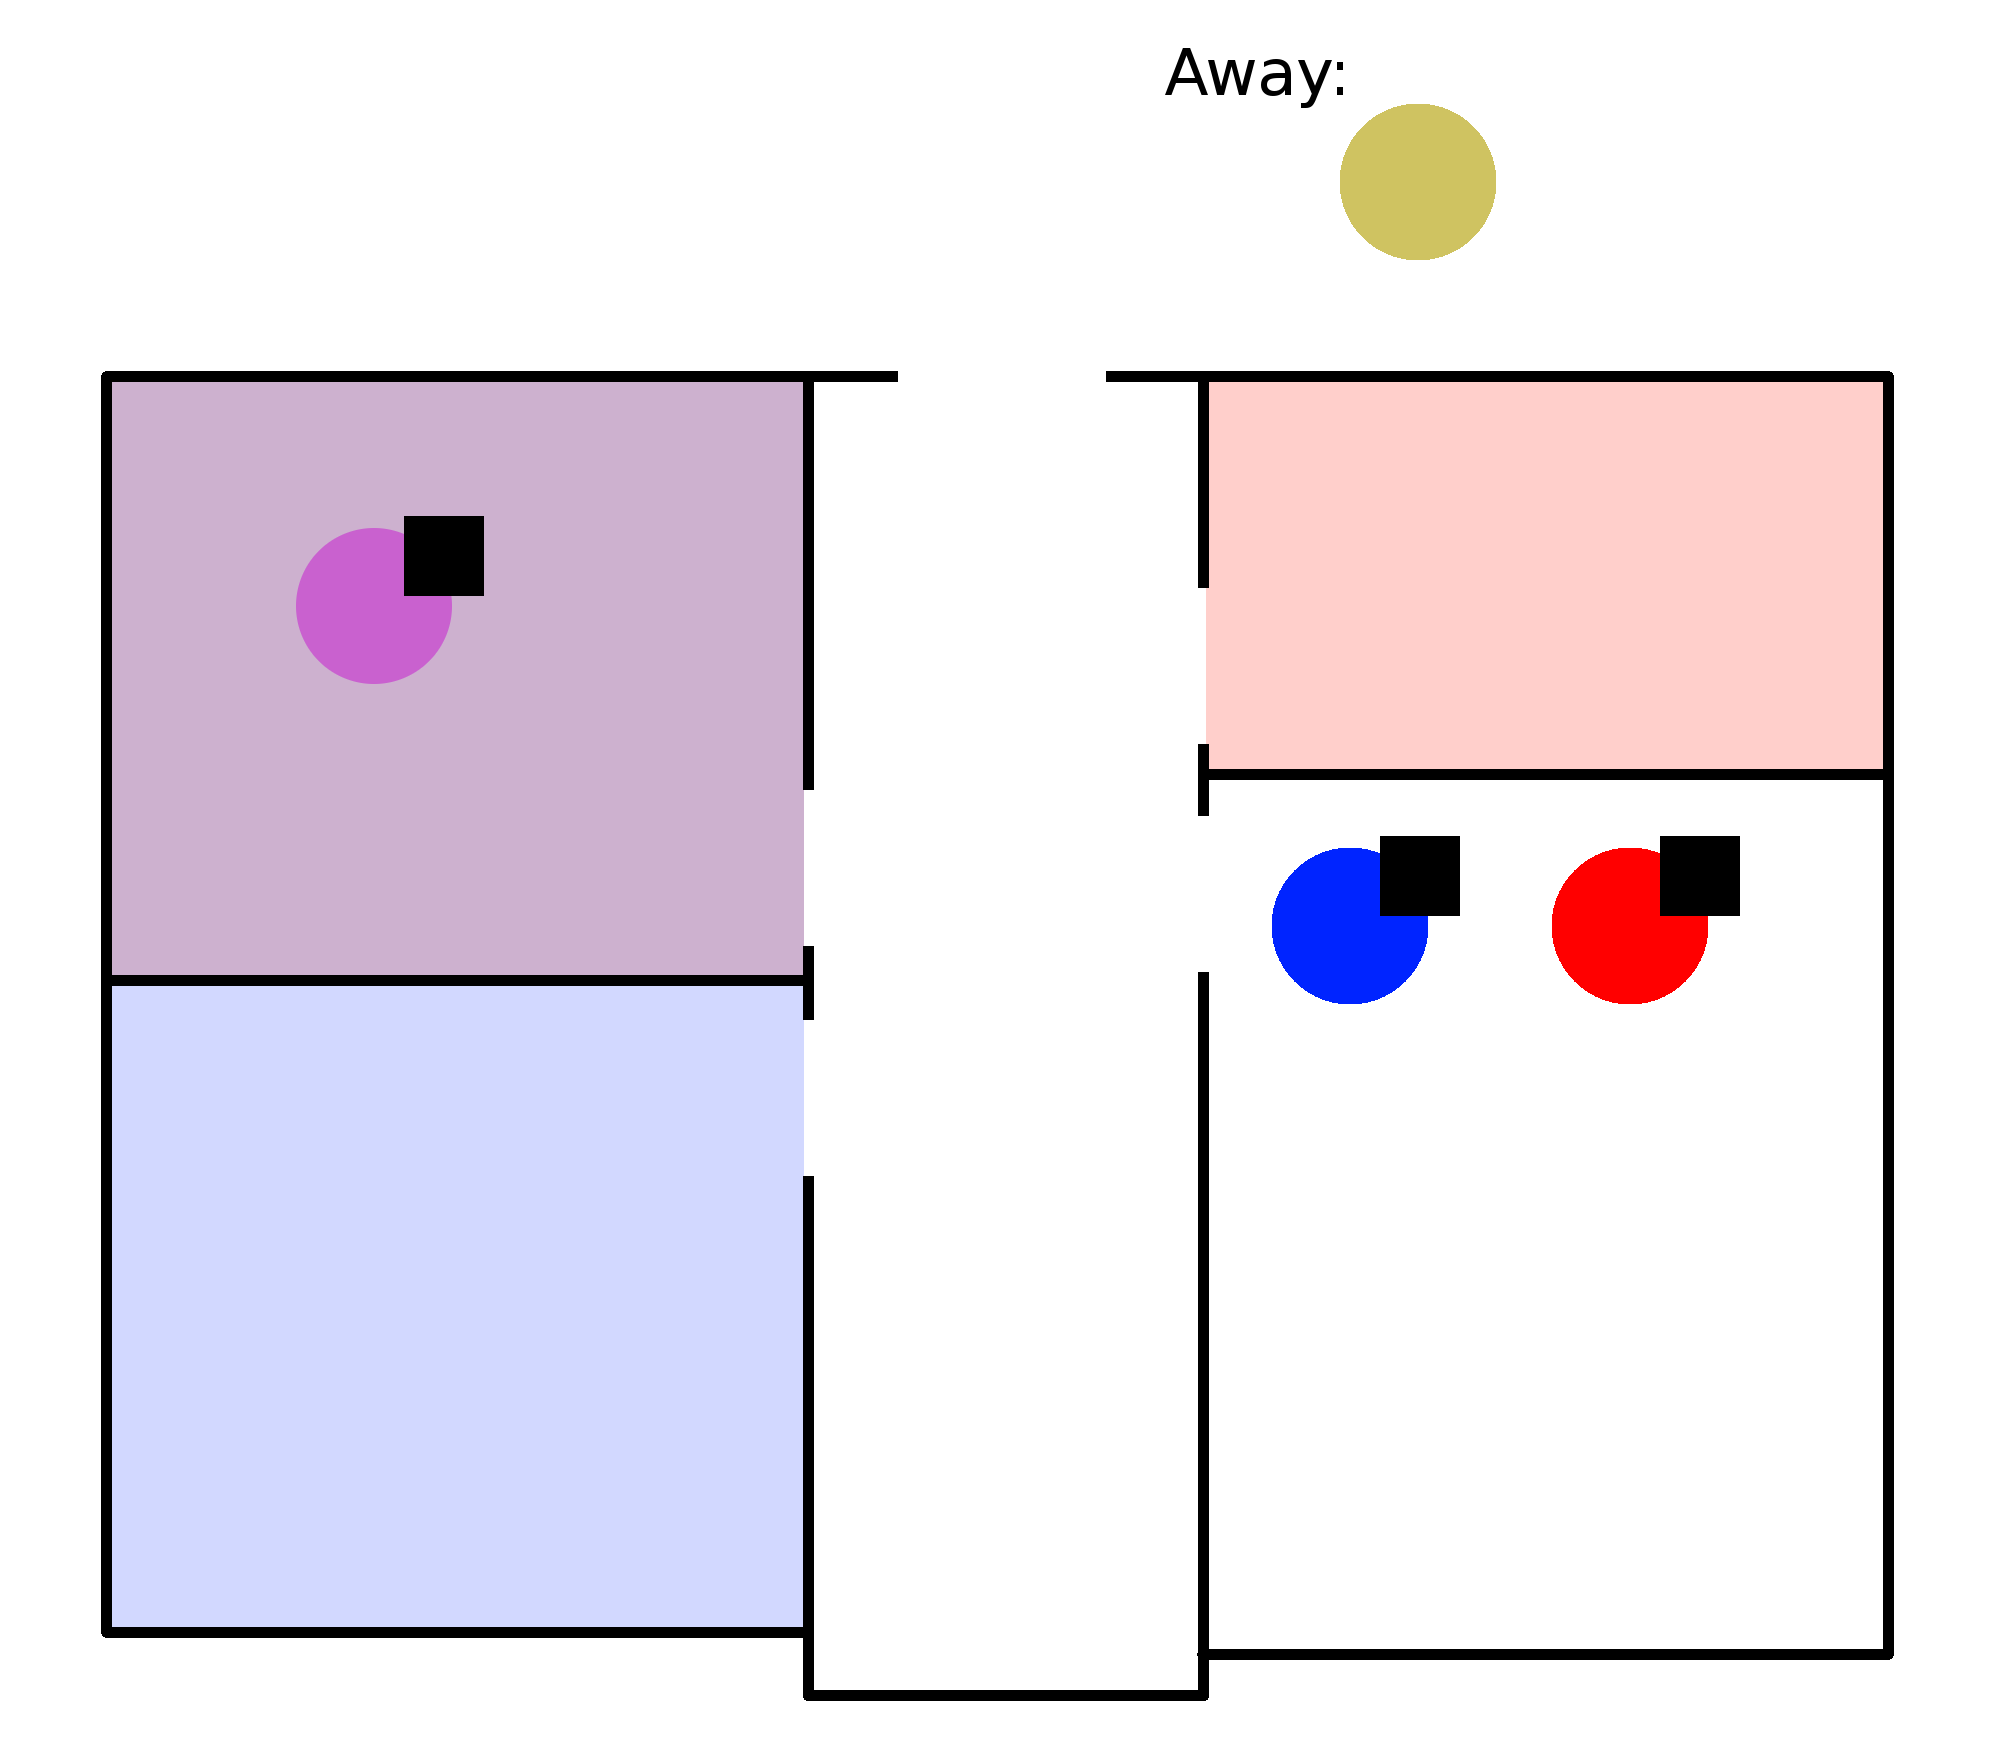
\includegraphics[width=\linewidth]{img/location_sharing}
	\caption[Location Sharing]{Location Sharing}
	\label{fig:location_sharing}
\end{figure}

The tracking is done using light sensors at doors reacting to people entering and leaving an office.
Then using wifi fingerprinting of the member's mobile device his location is determined.

Since the public display is placed within an office room, repeating changes on the screen my interrupt members working.
As consequence the display is dimmed when none is looking at it and changes are made using very smooth transitions.
Looking at the screen, the display lights up and its update frequency is increased.
This behavior is achieved using simple head tracking via camera and computer vision.

Concerning privacy not every member wants to be tracked all the time.
Also it must be possible to tell others not to be disturbed.
Therefore every member owns a configurable personal profile controlling his privacy wishes.
It allows setting different visibility stages such as hiding oneself from the system,
Showing one's general availability and his location.
The later two modes allow further adjustments such as setting 'Do not disturb'.
In any mode it is also possible to set messages such as 'currently in mensa' to notify other members of ones location when not in office.
Also the door can be used as input to control these modes.
An open door could represent availability and a closed unavailability or that the member is busy.

A web based administration interface is used to manage member-office associations.

As extension we propose to add a public display in front of the office to allow external persons such as students see which office member is currently available.
The setting if a student may see a persons availability is configured by each member individually in his privacy profile.



\subsection{Video Sharing}

todo

\subsection{Screencast Sharing}

The idea behind screen sharing is to provide a platform for displaying content from a personal device, such as a smartphone or notebook, on a public display.
The user can either share her/his whole screen or draw a bounding box, encompassing the to be shared content.
The purpose of sharing is solely to display the content, not to make the displayed information accessible e.g. in the matter of downloading data.
As a consequence, a high level of privacy is concomitant with screen sharing.
A user can share a section of her/his screen either from being located in the room with the public display where the content is intended to be displayed or while being situated in another room, e.g. her/his office.

In order to initiate screen sharing, the user configures the desired content and location in the client on the private device.
Additionally, combining screen sharing with video-chat is a possibility.

\begin{figure}
	\centering
	\includegraphics[width=\linewidth]{img/screensharing.png}
	\caption[Screen Sharing]{Shared content is marked with colored frames on the public display as well as the private devices.}
	\label{data_share_sequence}
\end{figure}

\subsection{Calendar Sharing}

By including the user’s calendar (e.g. Google Calendar) into a network of public displays (MIND), the functionality of the latter can be enriched.
The system may retrieve information from the calendar, such as meetings or not assigned timeslots.
For example can the system initiate conference calls or render the accessibility of the user in the system either busy or available, dependant on the calendar entries.
The effect of the calendar on the system can be adjusted by the user via a dedicated GUI.

\subsection{Data to Go}
\label{data2go}

One part of the proposed architecture would be location aware data sharing within the display network.
This is envisioned to work in two general modes, which are based on the underlying location sharing described in section \ref{location_sharing}.
The first would allow the pinning of data to a user's location, leaving its visibility set to private.
This would allow a user to take data with him when going to a colleagues' office for a meeting.
Apart from making the data available to the system, no further care would need to be taken to keep data readily available.
The second mode would allow data to be shared by sending it to a certain location, for example a meeting room.
This would make the data publicly available, primarily for that location.
Once that shared data is accessed from the location, its ownership would transfer away from its originating owner to a public ownership based on the location.

Figure \ref{data_share_sequence} shows some concepts for how the system would handle the data via the proposed modes.
Private sharing of data is also allowed by pinning data to another person.
This person then has access to the data based on their location, although ownership only transfers at a specific event that will have to be specified based on user preference and usage for download.

\begin{figure}
	\centering
	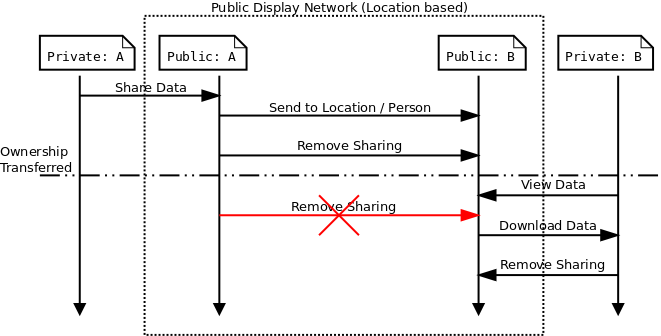
\includegraphics[width=\linewidth]{img/data_sharing.png}
	\caption[Data Sharing Sequence]{Informal sequence diagram of how data sharing might work, including some privacy and security options.}
	\label{data_share_sequence}
\end{figure}

As no data can be generated in the first iterations of the system (although such capabilities might well be added), a way to transfer data to and from the system will be required.
Such a way also makes sense from a user point of view, as the system is to be used alongside a broad range of private computers of the users.
To solve this data transfer gap, we propose a client program for a variety of devices that allows data control.
Pinning data to the user's own location (as in his private space) can be done by simply allowing the user to drag\&drop a file onto the client application, which will handle any conversion and transferring mechanism.
Similarly, retrieving data from a location or private area can be done by selecting the data via the client.
Having a client for not only desktop computers but also for smartphones would enable a broader and more comprehensive usage of the proposed service system.

% glossary
\section{Glossary}

\begin{itemize}
\item \textbf{Application:} Program for mainly a single purpose. In most cases also only a single user.
\item \textbf{Computer:} Hardware platform on which systems and applications are run.
\item \textbf{Direct and Indirect Interaction:} Direct interaction implies that the components of the user interface can be directly interacted with. Indirect 
\item \textbf{Multiple User Interaction:} The users interact with one device at the same time 
\item \textbf{Output - single/multi user:} how many users a single device can reach within its direct environment with a single output channel.
\item \textbf{Single User Interaction:} Only one user interacts with one device  at a specific time (but the users can change immediately)
\item \textbf{System:} Program for a multitude of tasks and purposes. Interacts with a variable number of users.
\item \textbf{Terminal device:} an output- (and most often also input-) device at either end of a communication link
\end{itemize}

\bibliographystyle{alpha}
\bibliography{sources}  

% use this to make sure that columns are balanced on the last page.
\balancecolumns

\end{document}
